\chapter{\label{cha:sts_transformers}Adopting Transformers for STS}

\section{Introduction}




Transformer models adopt a pre-training followed by fine-tuning scheme which means that once pre-trained these models can be fine-tuned to a large number of down-stream NLP tasks like text classification, named entity recognition etc.  Transformer models, which we have considered in this chapter use special tokens to obtain a single contiguous sequence for each input sequence. Specifically, the first token is always a special classification token \textsc{[CLS]} and sentence pairs are separated using a special token \textsc{[SEP]}. The final hidden state of \textsc{[CLS]}  is used for sentence-level fine-tuning tasks and the final hidden state of each token is used for token-level fine-tuning tasks. The fine-tuning scheme in transformers is usually simple like adding a softmax layer on top of \textsc{[CLS]} token for the text classification tasks. Furthermore, the fine-tuning scheme is very efficient as the parameters in the transformer model are already optimised with the pre-training process. Therefore, transformer models have been extremely popular and successful in many NLP tasks \cite{devlin-etal-2019-bert}. 

In this chapter, we explore different transformers models in variety of STS experiments. 
We address four research questions in this chapter:

\textbf{RQ1:} How well the existing state-of-the-art transformer models perform in STS task? 

\textbf{RQ2:} Can the method further improved with transfer learning and data augmentation techniques?

\textbf{RQ3:} Can the transformer model be easily adopted in to different languages?

\textbf{RQ4:} How well the proposed transformer models perform in a different domain? 

The main contributions of this chapter are as follows.

\begin{enumerate}
\item We evaluate five popular transformer models in three English STS datasets. We compare the results with the previous methods and show that transformer based STS methods outperform all the other STS methods we have experimented.

\item We propose further enhancements to the architecture using inter dataset transfer learning and data augmentation.  

\item We evaluate how well the transformer models perform on STS datasets in different languages and domains. 

\item The code and the pre-trained models are publicly available to the community\footnote{The public GitHub repository is available on \url{https://github.com/tharindudr/STS-Transformers}}. We have published the code as a python library \footnote{The developed python library is available on \url{https://pypi.org/project/ststransformers/}} and by the time of writing this chapter, it has more than 3,000 downloads from the community. 

\end{enumerate}

\section{Related Work}
As we mentioned before, after the introduction of BERT \cite{devlin-etal-2019-bert}, many variants of different transformer models have been proposed by adding minor modifications to the original BERT transformer. Usually these modifications has resulted in improvements in the fine-tuning scheme for the down-stream NLP tasks. Expecting a similar behaviour for the STS task too, we considered following transformer models for the experiments in this chapter.

\paragraph{BERT} \cite{devlin-etal-2019-bert} proposes a masked language modelling (MLM) objective, where some of the tokens of a input sequence are randomly masked, and the objective is to predict these masked positions taking the corrupted sequence as input. BERT applies a Transformer encoder to attend to bi-directional contexts during pre-training. In addition, BERT uses a next-sentence-prediction (NSP) objective. Given two input sentences, NSP predicts whether the second sentence is the actual next sentence of the first sentence. The NSP objective aims to improve the tasks, such as question answering and natural language inference, which require reasoning over sentence pairs. 

\paragraph{RoBERTa} \cite{liu2019roberta} makes a few changes to the BERT architecture and achieves substantial improvements. The changes include: (1) Training the model longer with larger batches and more data; (2) Removing the NSP objective; (3) Training on longer sequences; (4) Dynamically changing the masked positions during pre-training.

\paragraph{ALBERT} \cite{Lan2020ALBERT} proposes two parameter-reduction techniques (factorised embedding parameterisation and cross-layer parameter sharing) to lower memory consumption and speed up training. Furthermore, ALBERT \cite{Lan2020ALBERT} argues that the NSP objective in BERT lacks difficulty, as the negative examples are created by pairing segments from different documents, this mixes topic prediction and coherence prediction into a single task. ALBERT instead uses a sentence-order prediction
(SOP) objective. SOP obtains positive examples by taking out two consecutive segments and negative examples by reversing the order of two consecutive segments from the same document.


\paragraph{ELECTRA} Compared to BERT, ELECTRA \cite{Clark2020ELECTRA} proposes a more effective pre-training method. Instead of corrupting some positions of inputs with [MASK], ELECTRA replaces some tokens of the inputs with their plausible alternatives sampled from a small generator network. ELECTRA trains a discriminator to predict whether each token in the corrupted input was replaced by the generator or not. The pre-trained discriminator can then be used in downstream tasks for fine-tuning, improving upon the pre-trained representation learned by the generator.

\paragraph{XLNET} \cite{yang2019xlnet} identifies a key weakness in BERT pre-training. \citet{yang2019xlnet} argues that the symbols such as \textsc{[MASK]} that are introduced by BERT during pre-training, causes discrepancy between pre-training and fine-tuning as they never occur in real data. Therefore, XLNET suggests a new auto-regressive method based on permutation language modelling (PLM) \cite{JMLR:v17:16-272} without introducing any new symbols. 

Upon the introduction all of these transformer models have been evaluated in many down-stream NLP tasks including STS too. However, there is no comprehensive study done on STS using transformers considering big and small datasets, transfer learning, data augmentation, multilingual STS etc. which we do in this chapter.

\section{Transformer Architecture for STS}

The transformer architecture for STS is shown in Figure \ref{fig:sts_transformers}. The input of this model is a concatenation of the two sentences, separated by the \textsc{[SEP]} token. Then the output of the \textsc{[CLS]} token is used as the input of a softmax layer that predicts the similarity of the two sentences. We used mean-squared-error loss as the objective function. As the configurations, we used a batch-size of eight, Adam optimiser with learning rate $2\mathrm{e}{-5}$, and a linear learning rate warm-up over 10\% of the training data. During the training process, the parameters of the transformer, as well as the parameters of the subsequent layers, were updated. The models were trained using only training data. Furthermore, they were evaluated while training after each 100 batches, using an evaluation set that had one fifth of the rows in training data. We performed early stopping if the evaluation loss did not improve over ten evaluation steps. All the models were trained for three epochs. As these transformer models are computationally expensive, we used an Nvidia Tesla T4 GPU for the training process. We have kept these configuration same for all the experiments; in order to ensure consistency between all the languages and domains. This also provides a good starting configuration for researchers who intend to use transformers on a new language pair. The implementation is based on PyTorch \cite{NEURIPS2019_9015} and HuggingFace \cite{wolf-etal-2020-transformers}.

\begin{figure}[ht]
	\centering
	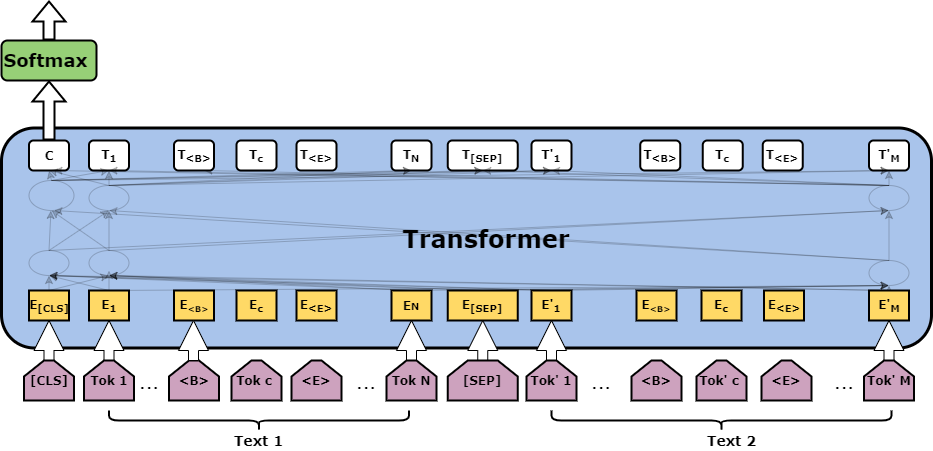
\includegraphics[scale=0.4]{figures/semantic_textual_similarity/transformers/STSTransformers.png}
	\caption[Architecture for using Transformers in STS]{Architecture for using Transformers in STS.}
	\label{fig:sts_transformers}
\end{figure}

\section{Exploring Transformers in English STS}
We evaluated all the above transformer variations in the three English STS datasets we introduced in \ref{cha:sts_introduction}; SICK, STS 2017 and QUORA. All of the transformer models we considered have several models that supports English (e.g.\ \textit{bert-large-cased} \& \textit{bert-base-cased} for BERT, \textit{text}).

 We trained the transformer models on the training sets on those datasets and evaluated them on the testing sets. 

The results are shown in Table \ref{tab:sick_transformers}, Table \ref{tab:sts_transformers} and Table \ref{tab:quora_transformers} respectively. 

\begin{table*}[htb]
	%\footnotesize
	\centering
	\scalebox{0.95}{
		\begin{tabular}{|l|cc|}
			\hline
			\textbf{Model} & $\bm{\rho}$   & $\bm{\tau}$     
			\\ \hline
			\textit{BERT}                  
			& 0.802 & 0.733  \\
			\hline
		\end{tabular}
	}
	\caption[Results for SICK with Transformer Models]{Results for SICK dataset with different variants of transformer models. For each variant, Pearson Correlation ($\bm{\rho}$) and Spearman Correlation ($\bm{\tau}$) are reported between the predicted values and the gold labels of the test set. Best result from all the variations is marked with ${\dagger}$.}  
	\label{tab:sick_transformers}
\end{table*}


\begin{table*}[htb]
	%\footnotesize
	\centering
	\scalebox{0.95}{
		\begin{tabular}{|l|cc|}
			\hline
			\textbf{Model} & $\bm{\rho}$   & $\bm{\tau}$     
			\\ \hline
			\textit{LSTM}                  
			& 0.831 & 0.762  \\
			\textit{Bi-LSTM}                     
			& 0.784 & 0.708   \\
			\textit{GRU}                     
			& 0.853$^{\dagger}$ & 0.811$^{\dagger}$  \\
			\textit{Bi-GRU}                     
			& 0.844 & 0.804  \\
			\textit{LSTM + Attention}                     
			& 0.830  & 0.791       \\
			\textit{GRU + Attention}                     
			& 0.825  & 0.782       \\
			\textit{GRU + Capsule + Flatten}                     
			& 0.806  & 0.765       \\
			\hline
		\end{tabular}
	}
	\caption[Results for STS 2017 with Transformers]{Results for STS 2017 dataset with different variants of Transformers. For each variant, Pearson Correlation ($\bm{\rho}$) and Spearman Correlation ($\bm{\tau}$) are reported between the predicted values and the gold labels of the test set. Best result from all the variations is marked with ${\dagger}$. }  
	\label{tab:sts_transformers}
\end{table*}


\begin{table*}[htb]
	%\footnotesize
	\centering
	\scalebox{0.95}{
		\begin{tabular}{|l|c|}
			\hline
			\textbf{Model} & RMSE     
			\\ \hline
			\textit{LSTM}                  
			& 0.412   \\
			\hline
		\end{tabular}
	}
	\caption[Results for QUORA with Transformers]{Results for QUORA dataset with different variants of Transformers. For each variant, Root Mean Squared Error (RMSE) reported between the predicted values and the gold labels of the test set. Best result from all the variations is marked with ${\dagger}$. }  
	\label{tab:quora_transformers}
\end{table*}


\subsection{Impact of Transfer Learning}

\subsection{Impact of Data Augmentation}



\section{Portability to Other Languages}

\section{Potability to Other Domains}

\section{Recent Developments: Siamese Transformers}

\section{Conclusions}